\chapter{Analisi}
In questo capitolo analizziamo la struttura del progetto, partendo dai suoi componenti e definendo la loro relazione.

%%%%%%%%%%%%%%%%%%%%%%%%%%%%%%%%%%%%%%%%%%%%%%%%%%%%%%%%%%%%%%%%
\section{Componenti}

\subsection{Task}
Un task è il template statico del sistema. È definito da: una deadline; un periodo; un sampler per l'execution tempo; una priorità nominale.

Non ci interessa definire un activation time perché vogliamo considerare il caso pessimo: l'activation time sarà uguale per tutti i task e coinciderà con l'istante iniziale.

\subsection{Job}
Un job rappresenta una singola istanza di esecuzione di un task. È l'entità dinamica che mantiene lo stato durante la simulazione. È definito da: il riferimento al task padre; il tempo di rilascio; la deadline assoluta; il tempo di esecuzione rimanente; la priorità dinamica.

\subsection{Taskset}
È un insieme di task. È l'oggetto principale gestito dallo scheduler.

\subsection{CPU}
È l'unità di elaborazione. Supponiamo essere unica.

\subsection{Scheduler}
È il componente che assegna un job al processore e gestisce l'avanzamento del tempo e il logging. Sono stati implementati Rate Monotonic (RM) e Earliest Deadline First (EDF).

%%%%%%%%%%%%%%%%%%%%%%%%%%%%%%%%%%%%%%%%%%%%%%%%%%%%%%%%%%%%%%%%
\section{Class diagram}
Per capire meglio la struttura del progetto, analizziamo il diagramma delle classi in Figura~\ref{fig:classDiagram}.

In questo modello sono definiti solo i campi che definiscono i vari componenti; per chiarezza del sistema non sono stati infatti introdotti gli oggetti necessari all'implementazione.
\begin{figure}[htbp]
    \centering
    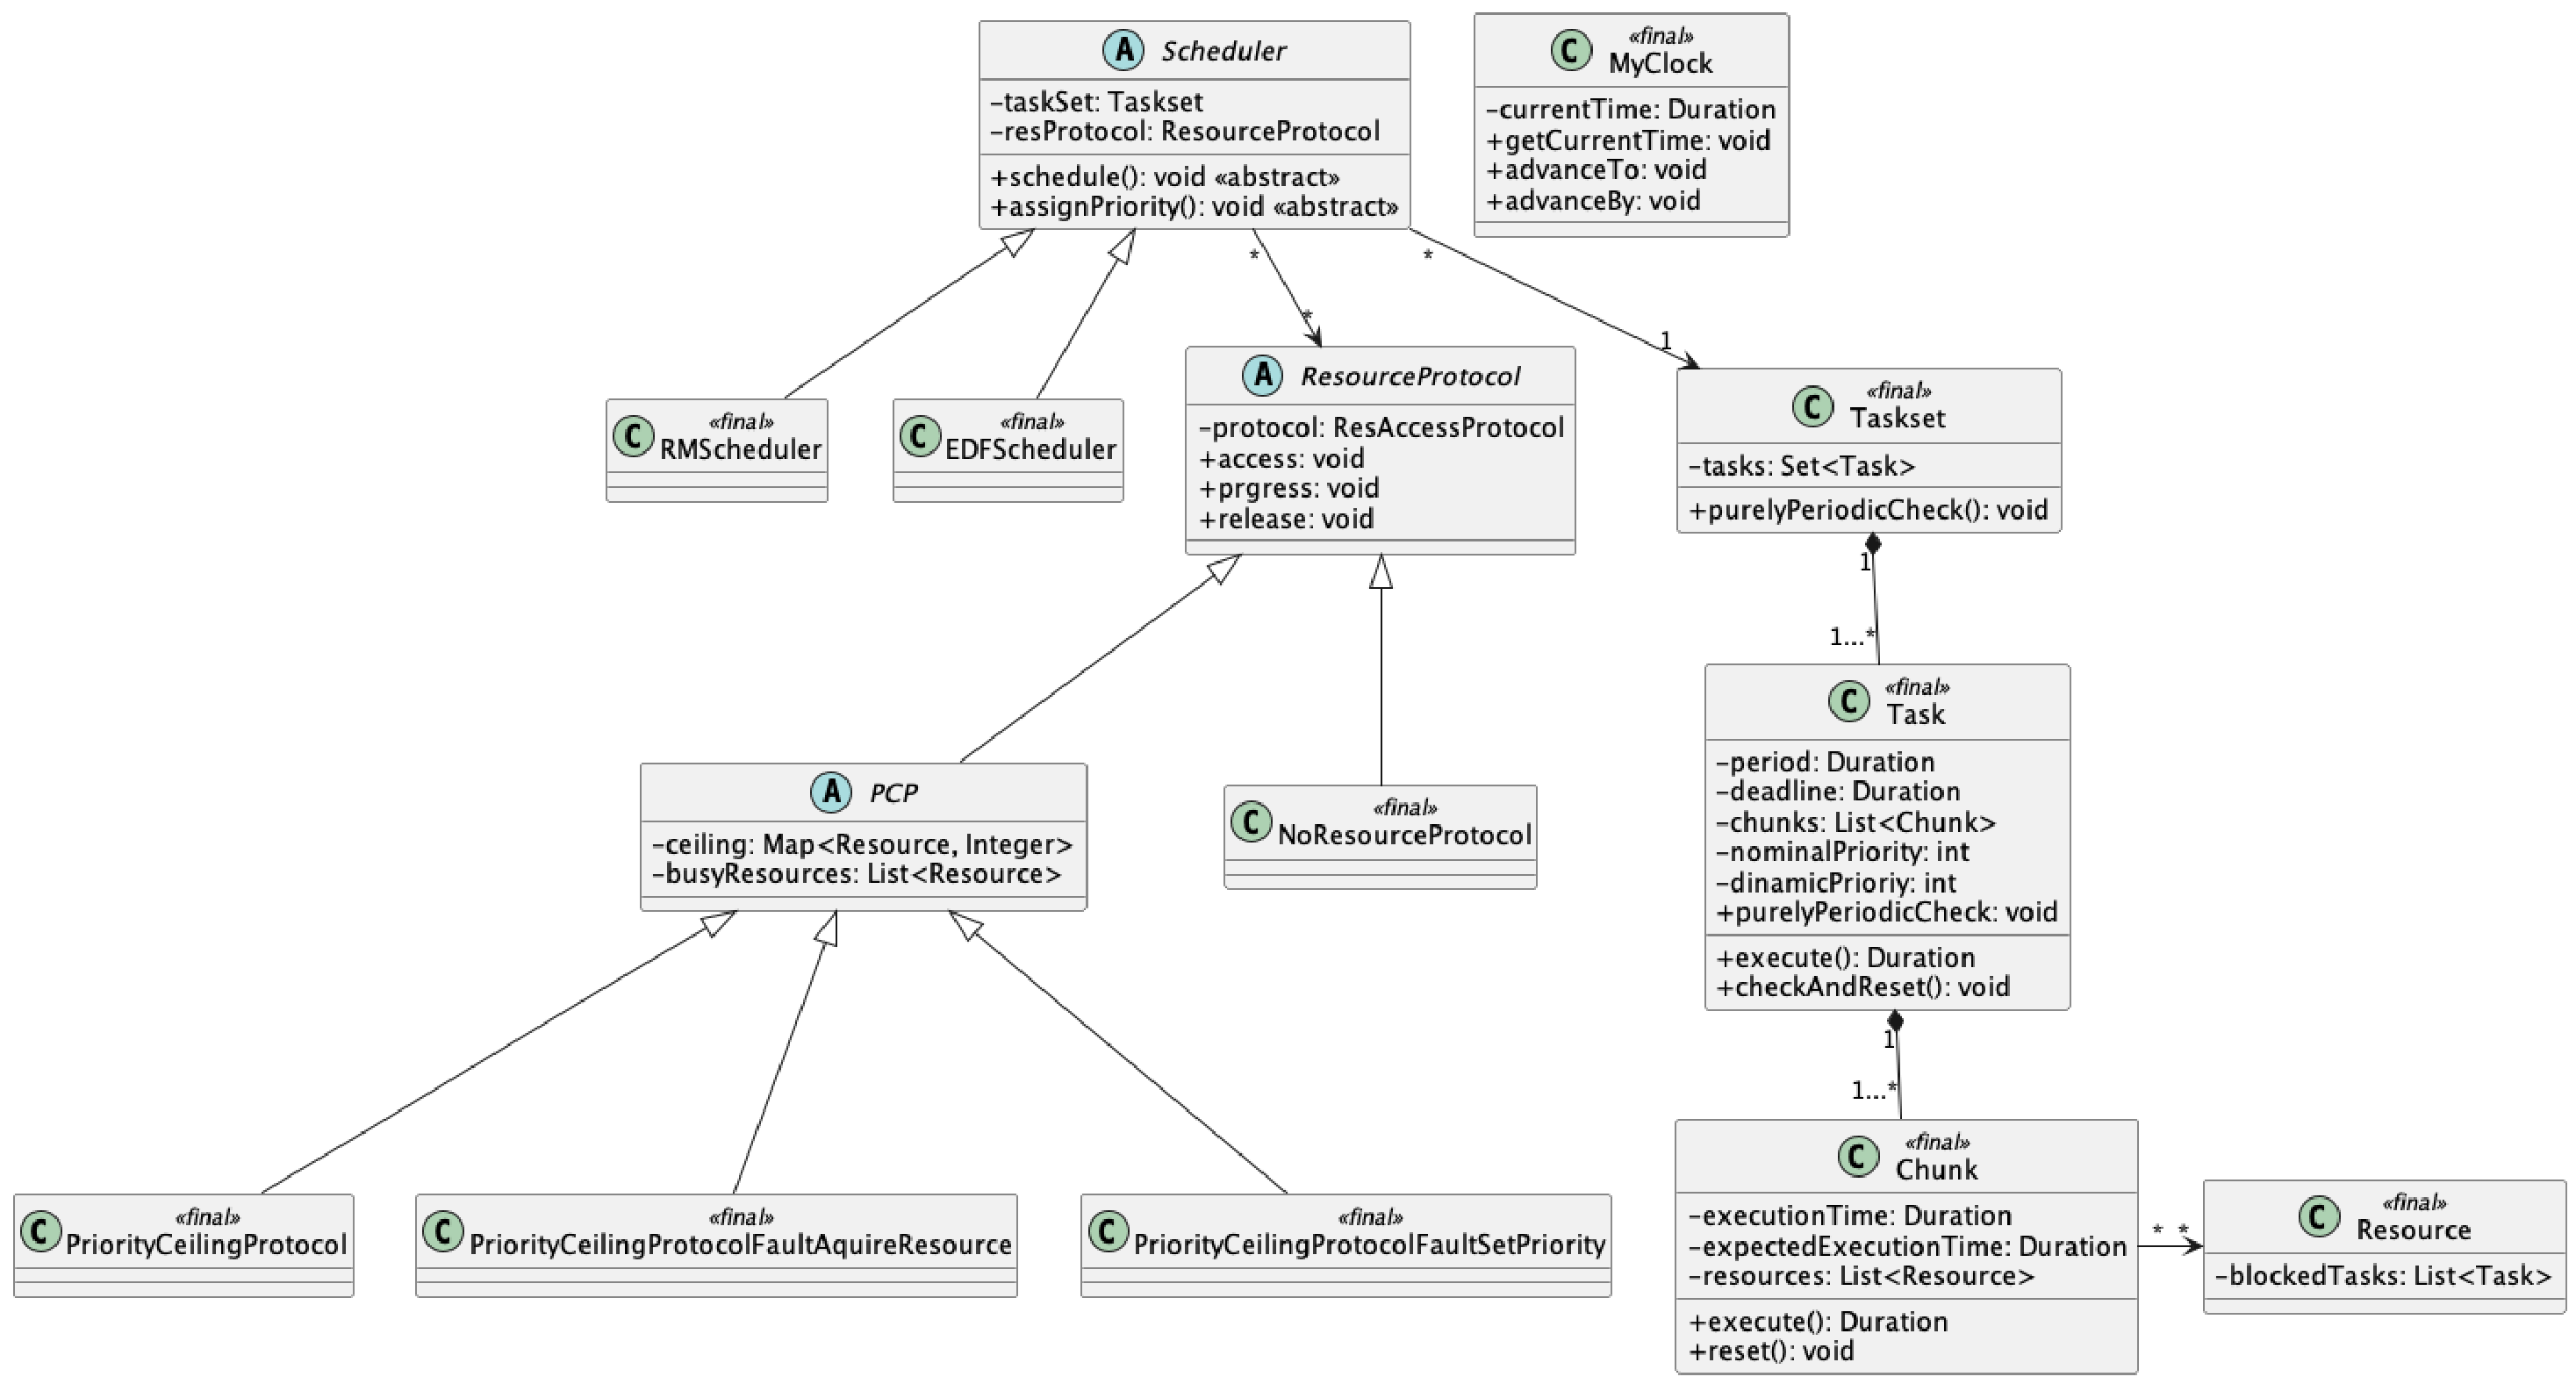
\includegraphics[width=1\textwidth]{immagini/class diagram.pdf}
    \caption{Class diagram}
    \label{fig:classDiagram}
\end{figure}